% Drawing 144/03-9 -- folder 144, batch 03, archive page 59 (PDF page 60).
% Transcription: Une sphère dont l'équateur porte les trois points $0$, $1$, $\infty$.
% Kind: sphere with three points on the equator. Method 2 (schematic redraw from the facsimile). Status: ok.
% Notes: Small sphere in the right margin: equator front solid, back dashed; 0 and 1 in front, infinity at the back. The label of the right-hand point is not legible; it is 1 by the transcription.
% Coordinates: 1 unit = 1 mm = 1/100 of the crop width (bbox in page fractions: [0.72, 0.31, 0.9, 0.42]).
% Redrawn by Claude (claude-opus-5-5), issue #73, 2026-11-07; not checked by a human; not compiled (no TeX in the session).
% Rights: reproduces part of the work -- behind RENDER_TRANSCRIPTS, never published by itself.
\documentclass[tikz,border=3pt]{standalone}
\usepackage{amsmath,amssymb}
\usetikzlibrary{patterns,arrows.meta}
\tikzset{pencil/.style={black!45}, struck/.style={black!35}, mark/.style={circle,draw,inner sep=1.3pt}, pt/.style={circle,fill,inner sep=0.9pt}, opt/.style={circle,draw,fill=white,inner sep=1.1pt}}
\begin{document}
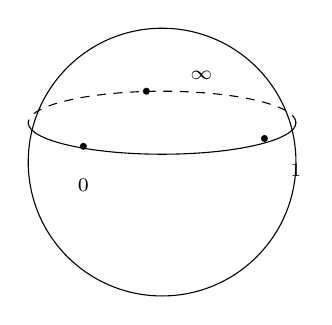
\begin{tikzpicture}[x=1mm,y=1mm,line cap=round,line join=round,font=\scriptsize]
\draw (57,-52) circle[radius=17];
\draw (40,-47) arc[start angle=180, end angle=360, x radius=17, y radius=4];
\draw[dashed] (74,-47) arc[start angle=0, end angle=180, x radius=17, y radius=4];
\node[pt] at (47,-50) {};
\node[pt] at (70,-49) {};
\node[pt] at (55,-43) {};
\node[inner sep=1pt] at (47,-55) {\scriptsize $0$};
\node[inner sep=1pt] at (74,-53) {\scriptsize $1$};
\node[inner sep=1pt] at (62,-41) {\scriptsize $\infty$};
\end{tikzpicture}
\end{document}
